\documentclass[a4paper,12pt]{article}

\usepackage[margin=1in]{geometry}
\usepackage{tikz}
\usepackage{amssymb}
\usepackage{xcolor}
\usepackage{circuitikz}
\usepackage{graphicx}

\newcommand{\ra}{$\rightarrow$}
\newenvironment{6mini}{
  \begin{minipage}{6cm}
}{
  \end{minipage}
}

\title{\texttt{Counters}\\\hrulefill}
\author{module 15}
\date{\small{11/23/2023}}

\begin{document}
    \maketitle

    \section{Counter \& Flip Flops}
        At a high level, a coutner is a logic device with a clock and multiple outputs (LSB \ra MSB).
        \begin{itemize}
            \item On the clock edge, the output will increment by one.
            \item once it reaches its max value (ex: 111) it will reset back to the starting value (000).
            \item They are designated b the size of their output: a 12 bit counterwould have 12 output bits.
            \item Are constructed with Flip Flops
        \end{itemize}
        T and JK flip flops will be utilized to construct a counter (JK can be constructed as a T). 

        \subsection{Counter}
            \texttt{Terminal count}: is the max counter can reach (all bits are 1). How fast it reaches said terminal cuont is a function of the clock
            \begin{itemize}
                \item A 1Hz clock will increment every second
                \item A 1 MHz clock will increment ever microsecond
            \end{itemize}
            \texttt{Resolution}: Difference in time between each count (the period of the clock $\frac{1}{F}$) is also a function of the clock.\\\\
            A higher bit counter can givemore counts, which can allow for more time to be represented. with the counter (i.e. delays).\\\\A faster clock will give greater resolution in time of the counter output.\\\\
            Flip flops connected together can perform a counting operation.
            \begin{itemize}
                \item Each clock increases the count
                \item Each flip flop is a bit in the count
                \item A 2 bit counter Counts 0 to 3, has 2 flip flops
                \item A 4 bit counter Counts 0 to 15, has 4 flip flops
                \item Counters roll oer at terminal count
            \end{itemize}

        \subsection{Asynchronous Counters}
            Counter were flip flops do not share a common clock
            \begin{itemize}
                \item Clock is conencted to the LSB flip flop only, output of flip flop is the output of the counter and the input of the next clock
                \item implemented with a seires of T flip flops (or equivalent using JK)
            \end{itemize}
            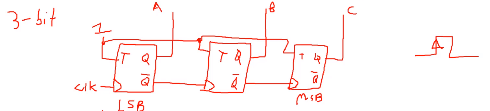
\includegraphics[width=12cm]{AsyncClock1.png}
            \subsubsection{Max frequency}
                The maximum frequency is determined by \textbf{propigation delay} of the flip flops and the number of flip flops used.
                \begin{itemize}
                    \item Clock cannot change faster than the time it takes for the last flip flop (MSB) output for the counter to change
                    \item If given a 4 bit counter, each with a 10 nanosecond delay, the fastest clock frequency would be $\frac{1}{40\textnormal{ns}}$.
                \end{itemize}

        \subsubsection{Synchronous Counters}
            All flip flops share the same clock, and the output of the previous flip flop is input to the next one.\\
            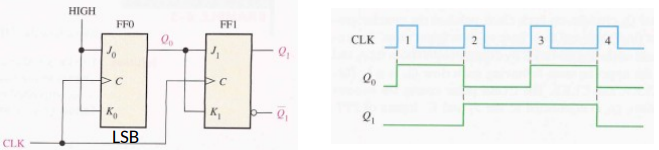
\includegraphics[width=12cm]{synchronousCounter1.png}\\
            In order to create larger synch counters, simply adding more flip flops would throw the count off.
            \begin{itemize}
                \item each additional digit will need an AND gate (excluding LSB \& MSB flip flop), which ANDs the flip flop output and input of said flip flop.
            \end{itemize}
            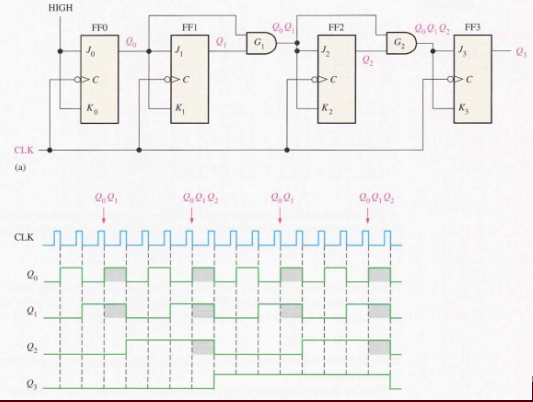
\includegraphics[width=10cm]{AddingDigits.png}\\
            The \textbf{max frequency} of the \underbar{counter} is determined by the max frequency that the \underbar{flip flop clocks can handle} \ra~There is no ripple effect from the clock.

    \section{Decade \& MOD counters}
            \subsection{Decade Counter}
                \begin{itemize}
                    \item Decade counter only counts 10 value, decimal 0 to 9.
                    \item utilizes NAND gates to reset flip flops
                    \item Outputs are used to reset the counter
                \end{itemize}
                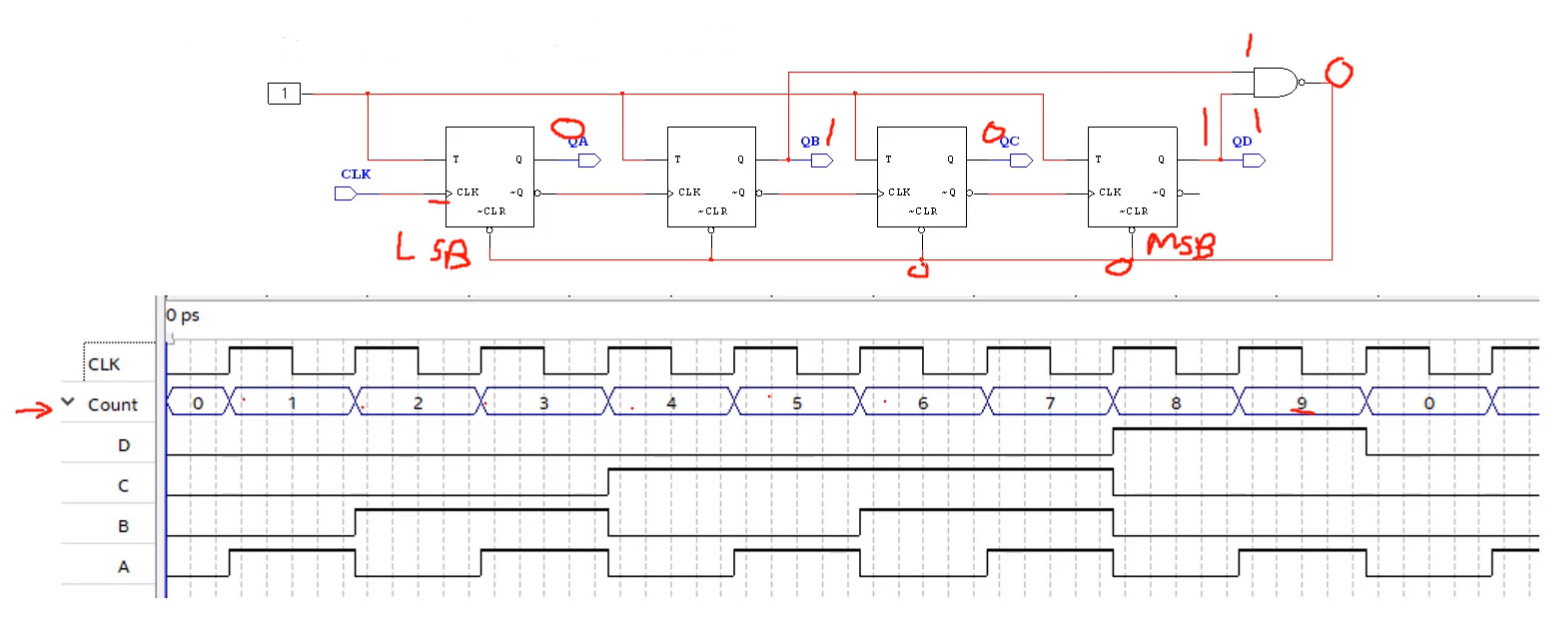
\includegraphics[width=15cm]{Decade1.png}\\\\
                A decade counte ris an exaple of a MOD counter (MOD 11 counter)
                
            \subsection{Modulus Counter}
                A MOD n counter only countains n counts.
                \begin{itemize}
                    \item MOD 4 counts 0 to 3
                    \item MOD 12 counts o to 11
                \end{itemize}
                Mod counters can also be made with state diagrams
\end{document}